%% 
%% Copyright 2007, 2008, 2009 Elsevier Ltd
%% 
%% This file is part of the 'Elsarticle Bundle'.
%% ---------------------------------------------
%% 
%% It may be distributed under the conditions of the LaTeX Project Public
%% License, either version 1.2 of this license or (at your option) any
%% later version.  The latest version of this license is in
%%    http://www.latex-project.org/lppl.txt
%% and version 1.2 or later is part of all distributions of LaTeX
%% version 1999/12/01 or later.
%% 
%% The list of all files belonging to the 'Elsarticle Bundle' is
%% given in the file `manifest.txt'.
%% 
%% Template article for Elsevier's document class `elsarticle'
%% with harvard style bibliographic references
%% SP 2008/03/01

\documentclass[preprint,12pt]{elsarticle}
%\documentclass[3p,12pt,authoryear]{elsarticle}

%% Use the option review to obtain double line spacing
%% \documentclass[authoryear,preprint,review,12pt]{elsarticle}

%% Use the options 1p,twocolumn; 3p; 3p,twocolumn; 5p; or 5p,twocolumn
%% for a journal layout:
%% \documentclass[final,1p,times,authoryear]{elsarticle}
%% \documentclass[final,1p,times,twocolumn,authoryear]{elsarticle}
%% \documentclass[final,3p,times,authoryear]{elsarticle}
%% \documentclass[final,3p,times,twocolumn,authoryear]{elsarticle}
%% \documentclass[final,5p,times,authoryear]{elsarticle}
%% \documentclass[final,5p,times,twocolumn,authoryear]{elsarticle}

\usepackage{hyperref}
\hypersetup{
  colorlinks   = true, %Colours links instead of ugly boxes
  urlcolor     = blue, %Colour for external hyperlinks
  linkcolor    = blue, %Colour of internal links
  citecolor   = red %Colour of citations
}

%% For including figures, graphicx.sty has been loaded in
%% elsarticle.cls. If you prefer to use the old commands
%% please give \usepackage{epsfig}
\usepackage{subfig}

%% The amssymb package provides various useful mathematical symbols
\usepackage{amssymb}
\usepackage{amsmath}
\usepackage{esint}
%% The amsthm package provides extended theorem environments
%% \usepackage{amsthm}

%% The lineno packages adds line numbers. Start line numbering with
%% \begin{linenumbers}, end it with \end{linenumbers}. Or switch it on
%% for the whole article with \linenumbers.
%% \usepackage{lineno}

\journal{Applied Mathematics and Computation}

%commands:
\newcommand{\fig}[1]{\hyperref[#1]{Fig.\ref{#1}}}
\newcommand{\figpath}{../graphics/}

%math:
\def\vc#1{\mathbf{\boldsymbol{#1}}}     % vector
\def\abs#1{\left|#1\right|}
\def\avg#1{\langle#1\rangle}
\def\d{\mathrm{d}}
\newcommand{\dd}{\; \mathrm{d}}
\newcommand{\R}{\mathbf{R}}
\newcommand{\bx}{\vc{x}}

\begin{document}

\begin{frontmatter}

%% Title, authors and addresses

%% use the tnoteref command within \title for footnotes;
%% use the tnotetext command for theassociated footnote;
%% use the fnref command within \author or \address for footnotes;
%% use the fntext command for theassociated footnote;
%% use the corref command within \author for corresponding author footnotes;
%% use the cortext command for theassociated footnote;
%% use the ead command for the email address,
%% and the form \ead[url] for the home page:
%% \title{Title\tnoteref{label1}}
%% \tnotetext[label1]{}
%% \author{Name\corref{cor1}\fnref{label2}}
%% \ead{email address}
%% \ead[url]{home page}
%% \fntext[label2]{}
%% \cortext[cor1]{}
%% \address{Address\fnref{label3}}
%% \fntext[label3]{}

\title{Partition of unity methods for approximation of point water sources in~porous media}

%% use optional labels to link authors explicitly to addresses:
%% \author[label1,label2]{}
%% \address[label1]{}
%% \address[label2]{}

\author[adr]{Pavel Exner\corref{cor1}}
\ead{pavel.exner@tul.cz}
\ead[url]{https://github.com/Paulie14/xfem\_project}
\cortext[cor1]{Corresponding author.}

\author[adr]{Jan B{\v r}ezina}
\ead{jan.brezina@tul.cz}

\address[adr]{Technical University of Liberec, Studentsk{\' a} 1402/2, 461 17 Liberec 1, Czech Republic}


\begin{abstract}
%% Text of abstract
In this work we demonstrate usage of Partition of Unity (PU) methods to improve approximation of singularities 
in the solution of the Poisson equation. Our model describes a steady flow of water in a system of aquifers
which consist of porous media. The aquifers are perforated by wells and boreholes which are often represented
as point sources considering their small diameter in comparision with the vast size of the aquifer. This 
brings singularities into the solution. The extended and stable generalized finite element method 
(XFEM and SGFEM) were implemented to solve the problem and a proper adaptive integration strategy was 
developed to gain optimal convergence rates.
\end{abstract}

\begin{keyword}
%% keywords here, in the form: keyword \sep keyword
PUM \sep XFEM \sep SGFEM \sep adaptive integration \sep point sources

%% PACS codes here, in the form: \PACS code \sep code

%% MSC codes here, in the form: \MSC code \sep code
%% or \MSC[2008] code \sep code (2000 is the default)

\end{keyword}

\end{frontmatter}

%% \linenumbers

%% main text
\section{Introduction}
\label{sec:introduction}

People often consider in their models of flow in porous media very large areas which can contain various 
phenomena of very small scale compared with the size of the areas. These can be some disruptions of the porous 
media, e.g. cracks and wells, or material inhomogeneities that cause large gradients in pressure head and 
velocity or even their discontinuities.

Using the standard finite element method (FEM) we are unable to properly approximate the quantities in the 
vicinity of these disturbances, unless we introduce elements of the same scale in the mesh. This leads to 
higher requirements on mesh processing (refinement) and increase of computational costs due to growing number  
of degrees of freedom.

In this work we use PU (Partition of Unity) methods to overcome these problems and demonstrate it on a steady 
%quasi-three-dimensional model of multi-aquifer system 
two-dimensinal aquifer model containing hydro-geological wells which cause singularities in solution. 
We follow the work \cite{gracie} and \cite{craig} who have already used the XFEM (eXtended FEM) on a~similar 
model. However, we focus mainly on the study of the PU methods. In particular, we use the XFEM and its 
corrected version (including ramp function and shift), e.g.~\cite{cxfem}, 
and the SGFEM, \cite{sgfem} and \cite{sgfem2013}. We are able to measure the convergence of pressure in $L^2$ 
norm over the aquifer domain and we compare the used methods. We also investigate the error of the
adaptive integration on the enriched elements and introcude improvement. In addition, we suggest better choice
of enrichment area based on a tolerance criterion.

The implementation was done in C++ language using the Deal II library~\citep{deal}, the finite element library.
which does not support any enrichment techniques at the moment.

We describe the model in the beginning of the article, set the problem and go through the
PU methods in more details. Then we show some numerical aspects of the problem which we must deal with, 
especially the adaptive integration in section \ref{sec:integration}. Results, convergence of methods and
conditioning of the algebraic system are discussed right after and further research goals are pointed out 
at the end. 

\section{Model}
\label{sec:model}
We consider a steady flow in a system of aquifers (2D layers of given thickness) which are separated by 
impermeable layers (aquitards). The aquifers are connected by wells which act as sources
or sinks in the domain of each aquifer. The pressure in the aquifers is further governed by the boundary 
condition of the aquifers which can be of Dirichlet type or be homogenous of Neumann type.

We describe the wells as interior boundary condition therefore we need to define the computational domain
as the aquifer domain with wells cross-sections cut off. Let the $\Theta^m$ be the domain on $m$-th aquifer,
$m=1,\ldots M$, $B^m_w$ be its cross-section with $w$-th well, $w\in\mathcal{W}=\{1,\ldots,W\}$, and denote
the union $B^m=\bigcup\limits_{w}B^m_w$. 
We then define domain $\Omega^m = \Theta^m\setminus B^m$ with an exterior boundary 
consisting of exclusive parts $\partial\Theta^m=\Gamma^m_D\cup\Gamma^m_N$ and an interior boundary 
$\partial B^m=\bigcup\limits_{w}\partial B^m_w$, such that $\partial\Omega^m=\partial\Theta^m\cup\partial B^m$.

The distribution of the pressure head in $m$-th aquifer is described by Poisson equation and 
boundary conditions
\begin{eqnarray} \label{eqn:poisson}
\nabla\cdot(-\mathbf{T}^m\nabla h^m) &=& f^m \qquad \textrm{on } \Omega^m\subset\R^2,\; \forall m=1,\dots,M, \\
h^m|_{\Gamma^m_D} &=& h^m_D, \\
\left(-\mathbf{T}^m\nabla h^m\cdot\vc{n}\right)|_{\Gamma^m_N} &=& 0, \\
\left(-\mathbf{T}^m\nabla h^m\cdot\vc{n}\right)|_{\partial B^m_w} &=& q^m_w \qquad \forall w\in\mathcal{W},
\end{eqnarray}
where $\mathbf{T}^m\, [\textrm{m}^2\textrm{s}^{-1}]$ denotes the transmisivity tensor,
%(we will further consider only scalar $T^m$ for simplicity), 
$h^m\, [\textrm{m}]$ the pressure head, $f^m\, [\textrm{m}\textrm{s}^{-1}]$ source density,
$\vc{n}$ unit normal vector on the boudnary and
$q^m_w = Q^m_w/|\partial B^m_w|$ is the density of the flow from the well to the aquifer over the well boundary 
$\partial B^m_w$. Equation \eqref{eqn:poisson} is derived from the Darcy law and the continuity equation 
for incompressible fluid.

Presuming the aquitards to be fully impermeable, the communication between aquifers is possible only through 
wells. We can prescribe the flow balance equation 
\begin{eqnarray}
  Q^m_w &=& Q^m_{w,in} - Q^m_{w,out}, \textrm{ where} \label{eqn:well_flows} \\
  Q^m_w &\ldots& \textrm{flow into aquifer across the well boundary,} \nonumber\\
  Q^m_{w,in} &\ldots& \textrm{flow from upper aquifer,} \nonumber\\
  Q^m_{w,out} &\ldots& \textrm{flow into lower aquifer.} \nonumber
\end{eqnarray}
\begin{figure}[!htb]
  %\vspace{-15pt}
  %TODO: add arrow (flow) to the top
  \begin{center}         
    \def\svgwidth{0.5\textwidth}
    \input{\figpath well_communcation.pdf_tex}
  \end{center}
  \caption{Flow balance in the well.}
  \label{fig:well_flows}
\end{figure}

\fig{fig:well_flows} presents the equation \eqref{eqn:well_flows} and denotes the flows $Q^m_{w,\cdot}$ by red arrows.
We can look at the flows in the balance equation as 1D problems which are governed by a difference of pressure
heads and a transition coefficient. Using this idea, we can substitute the flows in the equation 
\eqref{eqn:well_flows} and get
\begin{eqnarray} 
\int_{\partial B_w^m}\sigma_w^m \left(h^m - H_w^m\right) \dd s
  = c_w^{m+1}\left( H^m_w-H_w^{m+1}\right) - c^m_w\left( H^{m-1}_w-H^m_w \right), \label{eqn:well_balance} \\
 \forall m=1,\dots,M \textrm{ and } \forall w\in\mathcal{W}, \nonumber
\end{eqnarray}
where $\sigma^m_w\, [\textrm{m}\textrm{s}^{-1}]$ denotes the permeability coefficient between $w$-th well and 
$m$-th aquifer, $H_w^m$ the pressure head in the well $w$ at the level of $m$-th aquifer and finally 
$c^m_w\, [\textrm{m}^2\textrm{s}^{-1}]$ is the permeability of the well $w$ through aquitard $m$.

The problem is now to find set of functions $h^m\in C^2(\Omega^m)\cap{C}^1(\bar\Omega^m)$ and set of pressure 
values in the wells $H^m_w\in\R$, for all $m\in\{1,\ldots,M\}$ and $w\in\mathcal{W}$ that
satisfy the equations \eqref{eqn:poisson} and \eqref{eqn:well_balance}.

Note that if the lower end of well is considered isolated from below, the coefficient must be set $c^1_w = 0$.
With $c^m_w = 0$ we can also simulate the end of the well $w$ at the level of aquifer $m$.

We mention yet the equation \eqref{eqn:well_balance} for $m=M+1$ which is one level above the upmost aquifer
and is adjusted to the form
\begin{equation} \label{eqn:well_balance_top}
  c^M_w\left( H^{M}_w-H^{M+1}_w \right) = 0.
\end{equation}
The pressure at the top of the well $H^{M+1}_w$ can be set as an input value or, if not set, is gained 
as part of the solution from the equation \eqref{eqn:well_balance_top}, see $H^4$ in \fig{fig:well_flows}.

The boundary term in \eqref{eqn:well_balance} with large $\sigma^m_w$ would force the pressure head along the 
well edge to be constant (equal $H^m_w$), which cannot be in general satisfied. Therefore it is weakened and 
later replaced by the average
\begin{equation} \label{eqn:average}
  \avg{h^m} = \frac{1}{\abs{\partial B^m_w}} \int\limits_{\partial B^m_w} h^m \dd s,
\end{equation}
which corresponds to \cite{gracie}.

\subsection{Weak formulation}
We define the trial and the test spaces
\begin{eqnarray} \label{eqn:spaces}
  V &=& \prod\limits_{m=1}^{M}\big(H^1(\Omega^m)\times\R^W\big), \\
  V_0 &=& \prod\limits_{m=1}^{M}\big(H^1_0(\Omega^m)\times\R^W\big),
\end{eqnarray}
where $H^1$ and $H^1_0$ are standard Sobolev spaces and 
\[ H^1_0(\Omega^m)=\{\varphi\in H^1(\Omega^m); \varphi|_{\Gamma^m_D}=0\}. \]
We can now introduce the weak solution $u$ and test functions $v$
\begin{eqnarray} \label{eqn:solution}
   u &=& (h^1,\ldots, h^M, H^1_1,\ldots,H^{M+1}_W)\in V, \\
   v &=& (\varphi^1,\ldots, \varphi^M, \Phi^1_1,\ldots,\Phi^{M+1}_W)\in V_0.
\end{eqnarray}

To obtain the weak form we apply the standard Galerkin method on \eqref{eqn:poisson} and \eqref{eqn:well_balance}, 
we further substract the second equation from the first one, use \eqref{eqn:average} and get for $m=1,\ldots,M$
\begin{multline} \label{eqn:weak_form}
  \int \limits_{\Omega^m} T^m \nabla h^m \cdot \nabla \varphi^m \dd\bx
        + \sum \limits_{w\in \mathcal{W}} \sigma^m_w\left( \avg{h^m}-H^m_w\right)
          \left(\avg{\varphi^m}-\Phi^m_w\right) + \\
          + \sum\limits_{w\in\mathcal{W}} \Big[
          c_w^{m+1}\left( H^m_w-H_w^{m+1}\right)\Phi^m_w - c^m_w\left( H^{m-1}_w-H^m_w \right)\Phi^m_w \Big]= \\
  =\int \limits_{\Omega^m} f^m\varphi^m \dd\bx.
\end{multline}


% Denoting $a^m(\cdot, \cdot)$ a bilinear form 
% \begin{equation} \label{eqn:bilinear_form_a}
%   a^m(u,v) = \int \limits_{\Omega^m} T^m \nabla u \cdot \nabla v \dd\bx
%         + \sum \limits_{w\in \mathcal{W}} \int \limits_{B^m_w} \sigma^m_w u v \dd\bx,
% \end{equation}
% we can write the weak form of \eqref{eqn:poisson}
% \begin{equation}% \label{eqn:weak_form}
%   a^m(h^m,v^m) - \int_{B_w^m}\sigma_w^m H_w^m v^m \dd\bx
%   = \int \limits_{\Omega^m} f^mv^m% - \int \limits_{\Omega^m} T^m \nabla h^m_D \nabla v^m \dd\mathbf{x},
%   \quad \forall m=1,\ldots,M,
% \end{equation}
% where the functions $h^m$ and test functions $v^m$ are from standard Sobolev spaces $H^1_0(\Omega^m)$,
% considering $h^m|_{\partial\Omega^m}=0$ for simplicity.
% The unknowns $H^m_w$ in \eqref{eqn:well_balance} are constants thus we can imagine that the test functions of 
% $H^m_w$ are also constants, chosen to be equal one, and so \eqref{eqn:well_balance} is not modified.

\section{Discretization}
\label{sec:pum_methods}
We can now proceed to the choice of the enrichment and discretize the system of equations
\eqref{eqn:weak_form}.
Let's imagine that we have only one aquifer so we can omit the upper index $m$ in this section.
In fact, it is appropriate to do so in some notations of shape functions because we do consider the same 
triangulation for every aquifer in our implementation.

\subsection{Enrichment function}
The enrichment function in general can be obtained from the knowledge of the solution character or 
from the solution of a simple local problem which will provide us the function.
In our case the simple problem is finding pressure distribution in a circular domain $\Omega$ with one well 
placed at the center. It can be easily proved that the function
%
\begin{equation} \label{eqn:solution_form}
  h = a \log(r_w)+b
\end{equation}
%
is the solution of a Laplace equation $-T \Delta h = 0$, just by putting the function into the equation. 
Argument $r_w$ of the logarithm is the distance from the well center
%
\begin{equation*}
      r_w(\bx) = \|\bx - \xi_w\|= \sqrt{(x-x_w)^2+(y-y_w)^2}.
\end{equation*}
%
We see in \eqref{eqn:solution_form} the logarithmic dependence of the pressure head on the distance from 
the well. If we represented the well only by a~point, the pressure head would go to infinity while closing 
to the point (singularity $\lim \limits_{r\rightarrow 0} \log r= -\infty$). Instead, we keep in mind the
radius of the well $R_w$ and introduce (global) enrichment function
%
\begin{equation}
\label{eqn:enrich_func}
s_w(\bx) = 
  \begin{cases}
  \log(r_w(\bx)), & r_w > R_w\\
  \log(R_w), & r_w \le R_w\\
  \end{cases}.
\end{equation}
See \fig{fig:enrich_func}.
It is natural to use the same set of $s_w$ on each aquifer since they depends only on $r_w$ and the wells are 
placed at the same positions throughout the aquifers (we consider only vertical wells, perpendicular to aquifers).
%
% and its gradient
% \begin{equation} \label{eqn:xgrad_func}
% \nabla s_w(\bx) = 
%   \begin{cases}  
%     \frac{\bx - \bx_w}{r_w^2(\bx)} & r_w>R_w \\
%     0 & r_w \leq R_w
%   \end{cases}.
% \end{equation}

\begin{figure}[!htb]
  %\vspace{-15pt}
  %TODO: do not forget to replace the notation of the enrichment function
  \begin{center}         
    \def\svgwidth{0.5\textwidth}
    \input{\figpath enrich_func.pdf_tex}
  \end{center}
  \caption{The enrichment function.}
  \label{fig:enrich_func}
\end{figure}

%TODO: define enrichment zone    
    
\subsection{Partition of unity methods}
Let $N_\alpha(\bx)$, $\alpha\in\mathcal{I}=\{1,\ldots,N\}$ be the standard linear finite element shape 
functions associated with the node $\bx_\alpha$ of the triangulation. 
In \textbf{standard XFEM}, we write the solution in the form
\begin{equation} \label{eqn:xfem_standard_form}
  h(\bx) = \sum \limits_{\alpha\in\mathcal{I}}a_\alpha N_\alpha(\bx)
    + \sum \limits_{w\in\mathcal{W}} \sum \limits_{\alpha\in\mathcal{I}^e_w} b_{\alpha w} \phi_{\alpha w}(\bx),
\end{equation}
where $a_\alpha$ are the standard FE degrees of freedom and $b_{\alpha w}$ are degrees of freedom coming from
enrichment of the well $w$. The index set $\mathcal{I}^e_w$ includes all nodes enriched by the well $w$, which
means that we have several enrichment functions and each can enrich different nodes.
The local enrichment functions $\phi_{\alpha w}$ in \eqref{eqn:xfem_standard_form} are defined
in the following way
\begin{equation} \label{eqn:xfem_enrich}
    \phi_{\alpha w} = N_\alpha(\bx)L_{\alpha w}(\bx), \quad \alpha\in\mathcal{I}^e_w, w\in\mathcal{W},
\end{equation}
where simply the enrichment function $L_{\alpha w}(\bx) = s_w(\bx)$.
%TODO: define test functions, refer to the weak form

\subsubsection{Corrected XFEM}
The corrected XFEM \citep{cxfem} deals with the convergence problem on blending elements and 
introduces the \textbf{ramp function}
%\begin{equation} \label{eqn:ramp_function}
\begin{eqnarray} \label{eqn:ramp_function}
  G_w(\bx) &=& \sum \limits_{\alpha\in\mathcal{I}_w^e} N_\alpha(\bx)    \\
  &=& 
  \begin{cases}
    0 & \textrm{ on unenriched elements}    \\
    1 & \textrm{ on elements where all nodes are enriched}    \\
    ramp & \textrm{ on elements where some of the nodes are enriched}    \\
  \end{cases} \nonumber
%   \quad \textrm{ on } \tau, \textrm{ such that } \bx,\bx_\alpha\in\tau, \\
%   g_{\alpha w} &=&
%   \begin{cases}
%     1 & \textrm{ if } \alpha \textrm{ is enriched by } w \\
%     0 & \textrm{ otherwise. }
%   \end{cases}
\end{eqnarray}
%\end{equation}
It also extends the set of enriched nodes, denoted by $\mathcal{J}^e$, by enriching (unenriched) nodes 
on elements, where only some of the nodes are in $\mathcal{I}^e$. Thus $\mathcal{I}^e\subset\mathcal{J}^e$ 
and there are more enriched nodes.
The enrichment function changes into the form
\begin{equation} \label{eqn:xfem_ramp}
    L_{\alpha w} = G_w(\bx) s_{w}(\bx), \quad \alpha\in\mathcal{J}^e, w\in\mathcal{W}.
\end{equation}
They further suggests the \textbf{shifted} enrichment functions in order to preserve the property of standard 
FE approximation at nodes $h(\bx_\alpha)=a_\alpha$; the value at the node is equal the corresponding degree
of freedom. The enrichment functions must be then zero at the nodes which is satisfied in the form
\begin{equation} \label{eqn:xfem_shift}
    L_{\alpha w} = G_w(\bx) \left[s_w(\bx) - s_w(\bx_\alpha)\right],
    \quad \alpha\in\mathcal{J}^e, w\in\mathcal{W}.
\end{equation} 
The property of the shifted formulation enables us to prescribe Dirichlet boundary condition such that
$a_\alpha = h_D(\bx_\alpha)$.

For the purpose of this article, let's call the XFEM with ramp function \textbf{XFEM-r} and the shifted 
version \textbf{XFEM-s}, as we shall reference to them later.

\subsubsection{SGFEM}
Finally we present the \textbf{SGFEM}, according to \cite{sgfem2013}. The enrichment function is defined
as the substraction of the global enrichment function and its interpolation 
\begin{equation} \label{eqn:sgfem_enrich}
    L_{\alpha w} = \left[s_w(\bx) - \pi_\tau (s_w)(\bx)\right],
    \quad \textrm{ on } \tau,\; \alpha\in\mathcal{I}^e, w\in\mathcal{W}.
\end{equation} 
where the interpolantion $\pi_\tau$ is built using the finite element shape functions
associated with nodes $\mathcal{I}(\tau)$ of the element $\tau$
\begin{equation} \label{eqn:sgfem_interpolation}
    \pi_\tau (s_w)(\bx) = \sum\limits_{\beta\in\mathcal{I}(\tau)} s_w(\bx_\beta) N_\beta(\bx).
    %\quad \textrm{ on } \tau,\; \alpha\in\mathcal{I}^e, w\in\mathcal{W}.
\end{equation}
Of course $\alpha\in\mathcal{I}(\tau)$ in \eqref{eqn:sgfem_enrich}.
Notice that there are no additional enriched nodes on blending elements, like in $\mathcal{J}^e$ in 
\eqref{eqn:xfem_ramp} and \eqref{eqn:xfem_shift}, and no ramp function is involved.

% \subsection{Assembly}
% Having the enrichment functions defined, the enriched nodes set and the equations discretized, we can approach
% the assembly of the linear system. The system has this block pattern 
% \begin{equation}
%   \begin{pmatrix}
%   \mathbf{E}^{M+1} &               &                     & \bar{\mathbf{F}}^{M+1}   & &&&&\\
%                    & \mathbf{K}^M  & \bar{\mathbf{R}}^M  & \bar{\mathbf{C}}^M       & &&&&\\
%                    & \mathbf{R}^M  & \mathbf{S}^M        & \bar{\mathbf{D}}^M       & &\ddots&&&\\
%   \mathbf{F}^{M+1} & \mathbf{C}^M  & \mathbf{D}^M        & \mathbf{E}^M             & &&&&\\
%   &&&& \ddots &&&& \\
%   &&&& & \mathbf{E}^2 &              &                    & \bar{\mathbf{F}}^2 \\
%   &&&\ddots& &              & \mathbf{K}^1 & \bar{\mathbf{R}}^1 & \bar{\mathbf{C}}^1 \\
%   &&&& &              & \mathbf{R}^1 & \mathbf{S}^1       & \bar{\mathbf{D}}^1 \\
%   &&&& & \mathbf{F}^2 & \mathbf{C}^1 & \mathbf{D}^1       & \mathbf{E}^1 \\
%   \end{pmatrix}
%   \begin{pmatrix}
%     \mathbf{H}^{M+1} \\
%     \mathbf{a}^{M} \\
%     \mathbf{b}^{M} \\
%     \mathbf{H}^{M} \\
%     \mathbf{\vdots} \\
%     \mathbf{H}^{2} \\
%     \mathbf{a}^{1} \\
%     \mathbf{b}^{1} \\
%     \mathbf{H}^{1} \\
%   \end{pmatrix} =
%   \begin{pmatrix}
%     \mathbf{f}^{M+1}_H \\
%     \mathbf{f}^{M}_a \\
%     \mathbf{f}^{M}_b \\
%     \mathbf{f}^{M}_H \\
%     \mathbf{\vdots} \\
%     \mathbf{f}^{2}_H \\
%     \mathbf{f}^{1}_a \\
%     \mathbf{f}^{1}_b \\
%     \mathbf{f}^{1}_H \\
%   \end{pmatrix}
% \end{equation}
% where $\mathbf{K}^m$ is the matrix of the standard FE approximation, $\mathbf{S}^m$ is the matrix of the 
% enrichment, $\mathbf{R}^m$ relates standard FE and enrichment,  $\mathbf{E}^m$ is the matrix associated with 
% unknown pressures in the wells and 
% $\mathbf{C}^m$, $\mathbf{D}^m$ and $\mathbf{F}^m$ are communication matrices: standard FE -- well, 
% enrichment -- well and well -- well, respectively. The whole system is symmetric.
% 
% The entries of the matrices are 
% 
% \begin{eqnarray}
%   K^m &=& \left[a^m(N^m_\alpha, N^m_\beta)\right]   ,\qquad \forall \alpha,\beta\in \mathcal{I} \label{eqn:k_entry}\\
%   S^m &=& \left[a^m(\phi^m_{\alpha k}, \phi^m_{\beta j})\right]     ,\qquad \forall \alpha,\beta\in \mathcal{I}^e,\; \forall k,j\in\mathcal{W} \label{eqn:s_entry}\\
%   R^m &=& \left[a^m(N^m_{\alpha}, \phi^m_{\beta j})\right]      ,\qquad \forall \alpha\in \mathcal{I},\; \forall\beta\in\mathcal{I}^e,\; \forall j\in\mathcal{W} \label{eqn:r_entry}\\
%   C^m_{w\alpha} &=&-\int\limits_{B^m_w} \sigma^m_w N^m_\alpha   ,\qquad \forall \alpha\in \mathcal{I},\; \forall w\in\mathcal{W}\\
%   D^m_{w\alpha j} &=&-\int\limits_{B^m_w} \sigma^m_w \phi^m_{\alpha j}  ,\qquad \forall \alpha\in \mathcal{I}^e,\; \forall w\in\mathcal{W}\\
%   \rm{diag}(\mathbf{E}^m)_w &=&\int\limits_{B^m_w} \sigma^m_w + c^{m+1}_w   ,\qquad \forall w\in\mathcal{W}\\
%   \rm{diag}(\mathbf{F}^m)_w &=& -c^m_w ,\qquad \forall w\in\mathcal{W}
% \end{eqnarray}

\section{Integration on enriched elements}
\label{sec:integration}
In order to compute the entries of the system matrix, %\eqref{eqn:s_entry} and \eqref{eqn:r_entry} 
we need to integrate
the expressions containing the enrichment functions. These of course can be non-polynomial, like they are 
in our case. The standard quadrature rules are not appropriate any more, as they are constructed to integrate 
precisely polynomials up to a given degree. The higher requirements on integration precision
are the price for using enrichment functions and a coarse mesh.

There are two aspects which the integration must handle properly:
\begin{itemize}
  \item the steep gradient of the pressure head in the vicinity of a well (the singularity),
  \item the well edge (since the elements of the triangulation do not take the well into account)
\end{itemize}

%TODO: better quadrature for log is not proper in our case as the function may be different according to hydrogeologist
One of the approaches to improve integration is local element refinement. We remind that the refinement only enables
placing more quadrature points in the element and does not bring any more degrees of freedom in the 
system. We will discuss the criterions for adaptive refinement, suggest improvement and compare our solution
with the original one in this subsection. We will refer also some of the convergence results which will be 
shown later in \ref{sec:results}.

\subsection{Adaptive refinement of an element}
\label{sec:refinement_element}

\cite{gracie} used a criterion for adaptive refinement according to which only the subelements 
that have nonzero cross-section with the well are refined. This catches nicely the well edge but it can work 
well only in some special cases when the well is at the node of an element or near the center of an element. 
The problem comes when the well is placed near the edge or node of an element. In that case there can be
large difference in the size of neighbouring subelements as you can see in \fig{fig:adapt_ref_a}. Although
the integrand is computed precisely enough on the element with the well inside, the quadrature points on the
neighbouring elements (where the pressure head gradient can be still large) are placed very sparsely 
and the integration error is large.

\begin{figure}[!htb]
%   \vspace{0pt}
  \centering    
  \subfloat[original refinement]{\label{fig:adapt_ref_a} 
    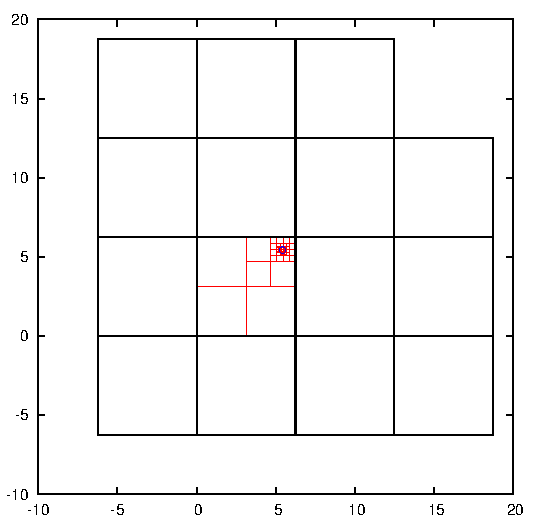
\includegraphics[width=0.45\textwidth]{results/adaptive_refinement_3_old.pdf} }
  \hspace{0pt}
  \subfloat[improved refinement]{\label{fig:adapt_ref_b} 
    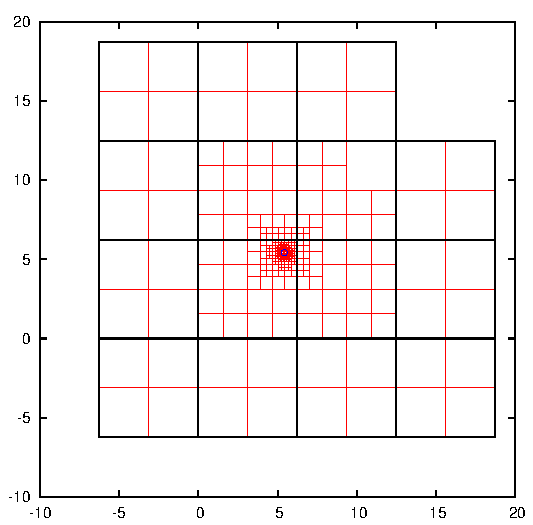
\includegraphics[width=0.45\textwidth]{results/adaptive_refinement_3_new.pdf} }
  \caption[Adaptive refinement comparision]
  {Comparision of the original and improved refinement techniques.
   Black lines denote enriched element edges, red lines denote adaptive refinement (subelement edges) and the well
   edge is blue.
  }
  \label{fig:adapt_refinement}
\end{figure}

We suggested additional criterion for subelements refinement which takes into account a subelement diameter 
and its distance from the well
\begin{equation}
  d_T > C_R|d_{min} - r_w|,
\end{equation}
where $d_T$ is the diameter of the subelement and $d_{min}$ is minimal distance between a vertex of 
the subelement and the well edge. $C_R$ is a scaling constant, equal 1.0 by default, through which we can 
control the significance of the criterion.

In this way, the elements in which the well does not lie are also refined as you can see in 
\fig{fig:adapt_ref_b}. The quadrature points are then distributed more 'smoothly' around the well and the
integrals with gradients can be computed more accurately. 

In \fig{fig:adapt_refinement_norm} you can see the $L_2$ norms of the error on the enriched elements which 
were computed also using the corresponding adaptive integration. Notice the scale of the improved version -- 
the error on elements is in small range and is not significantly concentrated anywhere. On the other hand, 
the original version shows out large error that is concentrated on the closest non-refined element to the well.

\begin{figure}[!htb]
%   \vspace{0pt}
%TODO: add axis, remove legend label, try to sharpen
  \centering    
  \subfloat[original refinement]{\label{fig:adapt_ref_norm_a} 
    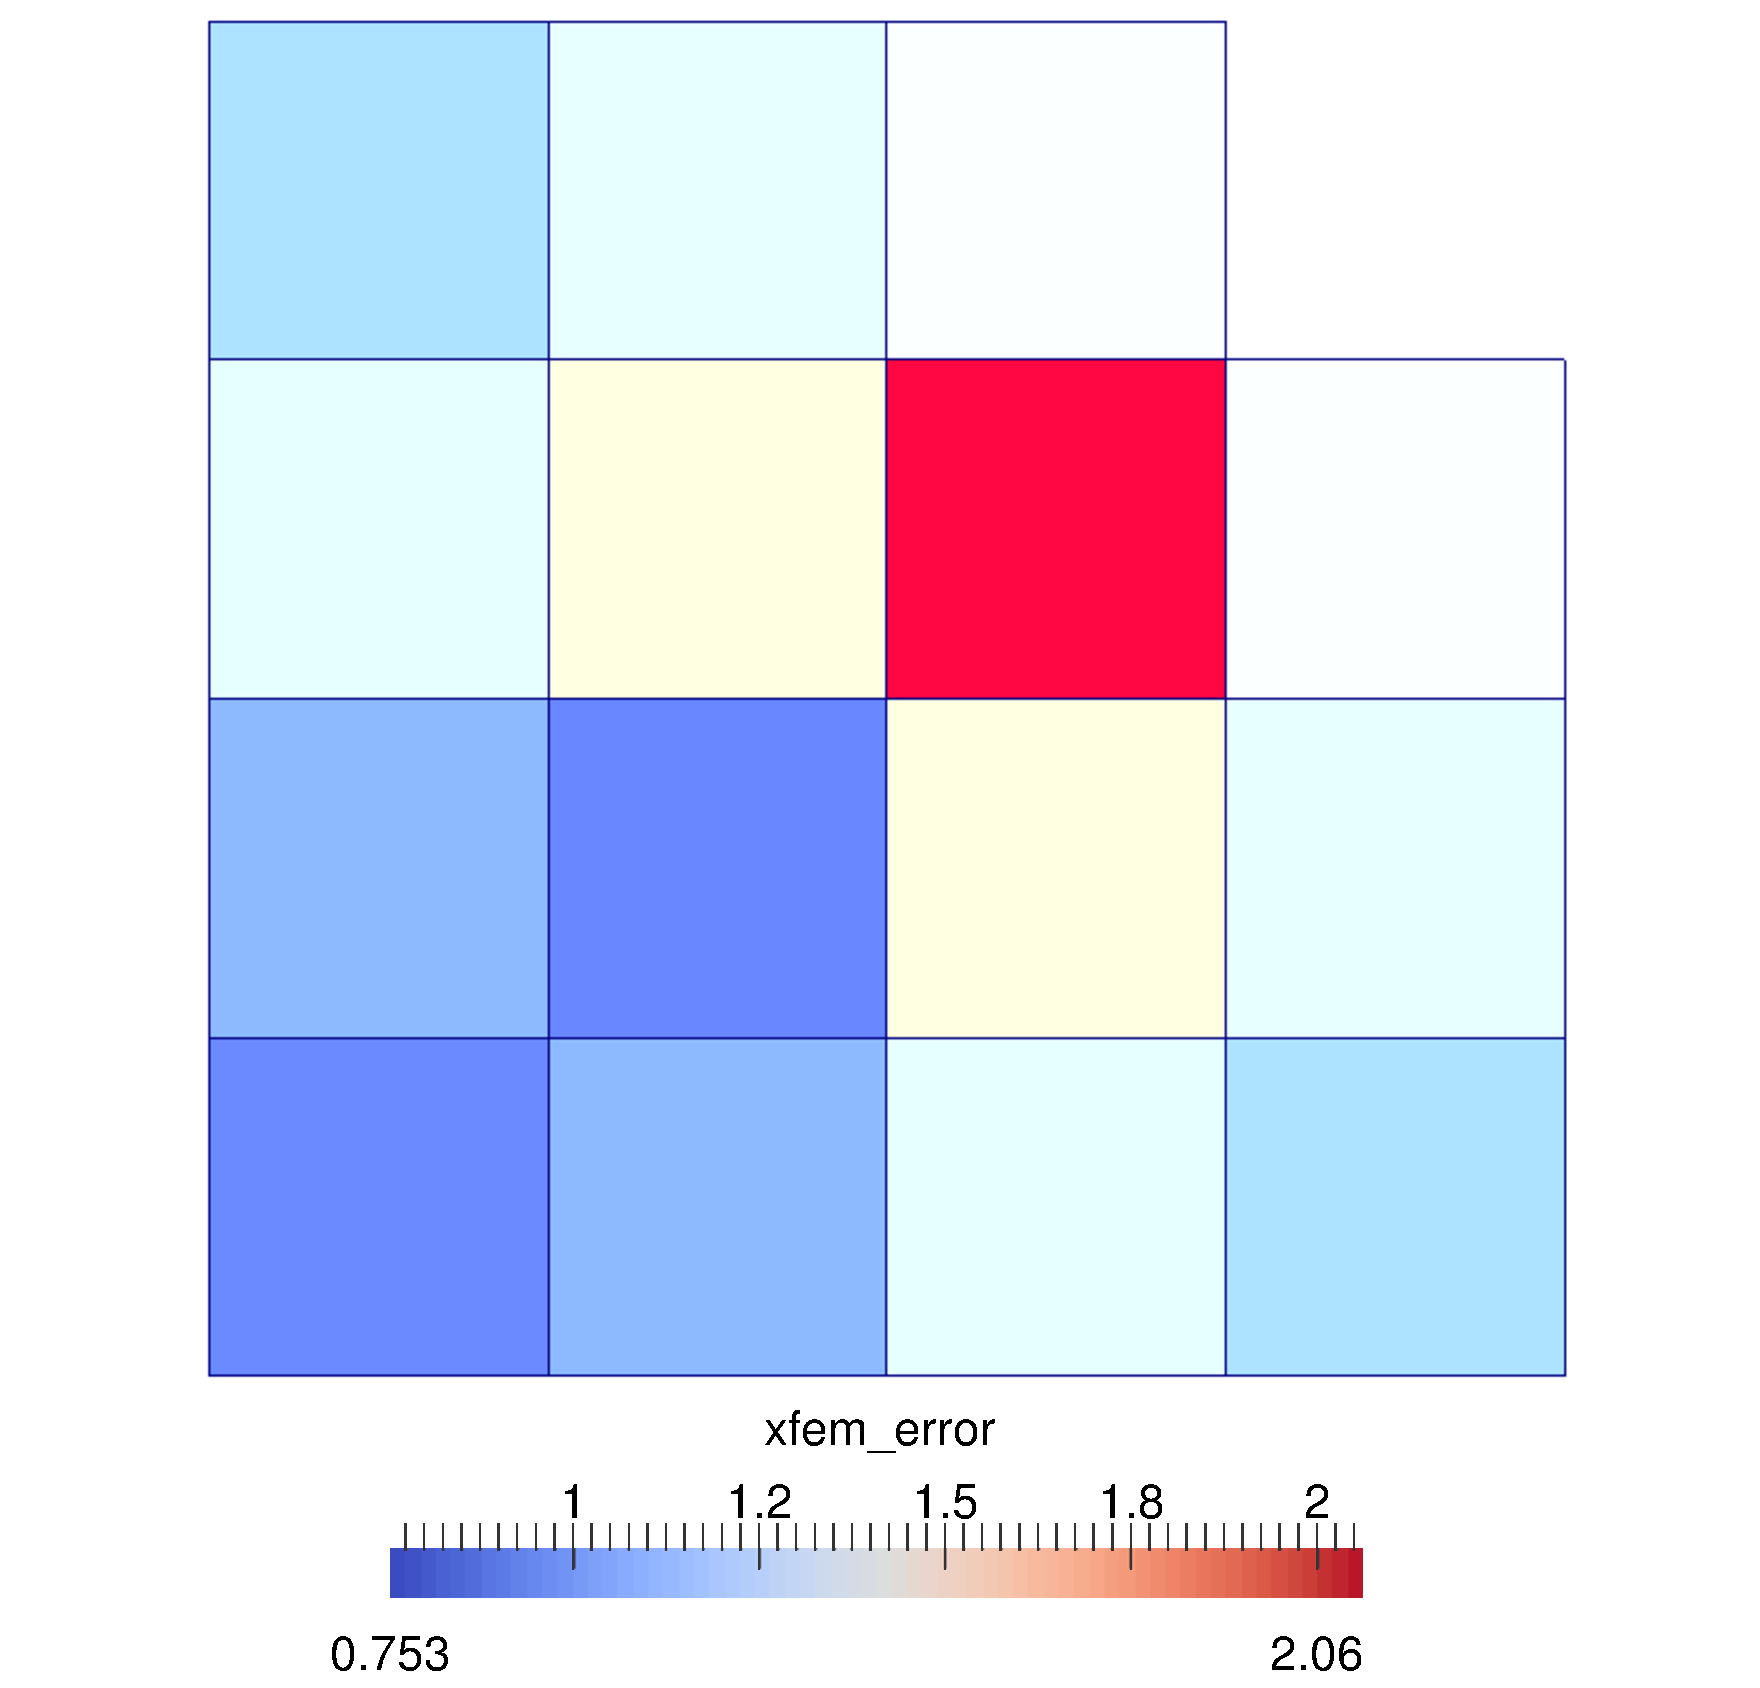
\includegraphics[width=0.45\textwidth]{results/adaptive_refinement_extract_3_old.pdf} }
  \hspace{0pt}
  \subfloat[improved refinement]{\label{fig:adapt_ref_norm_b} 
    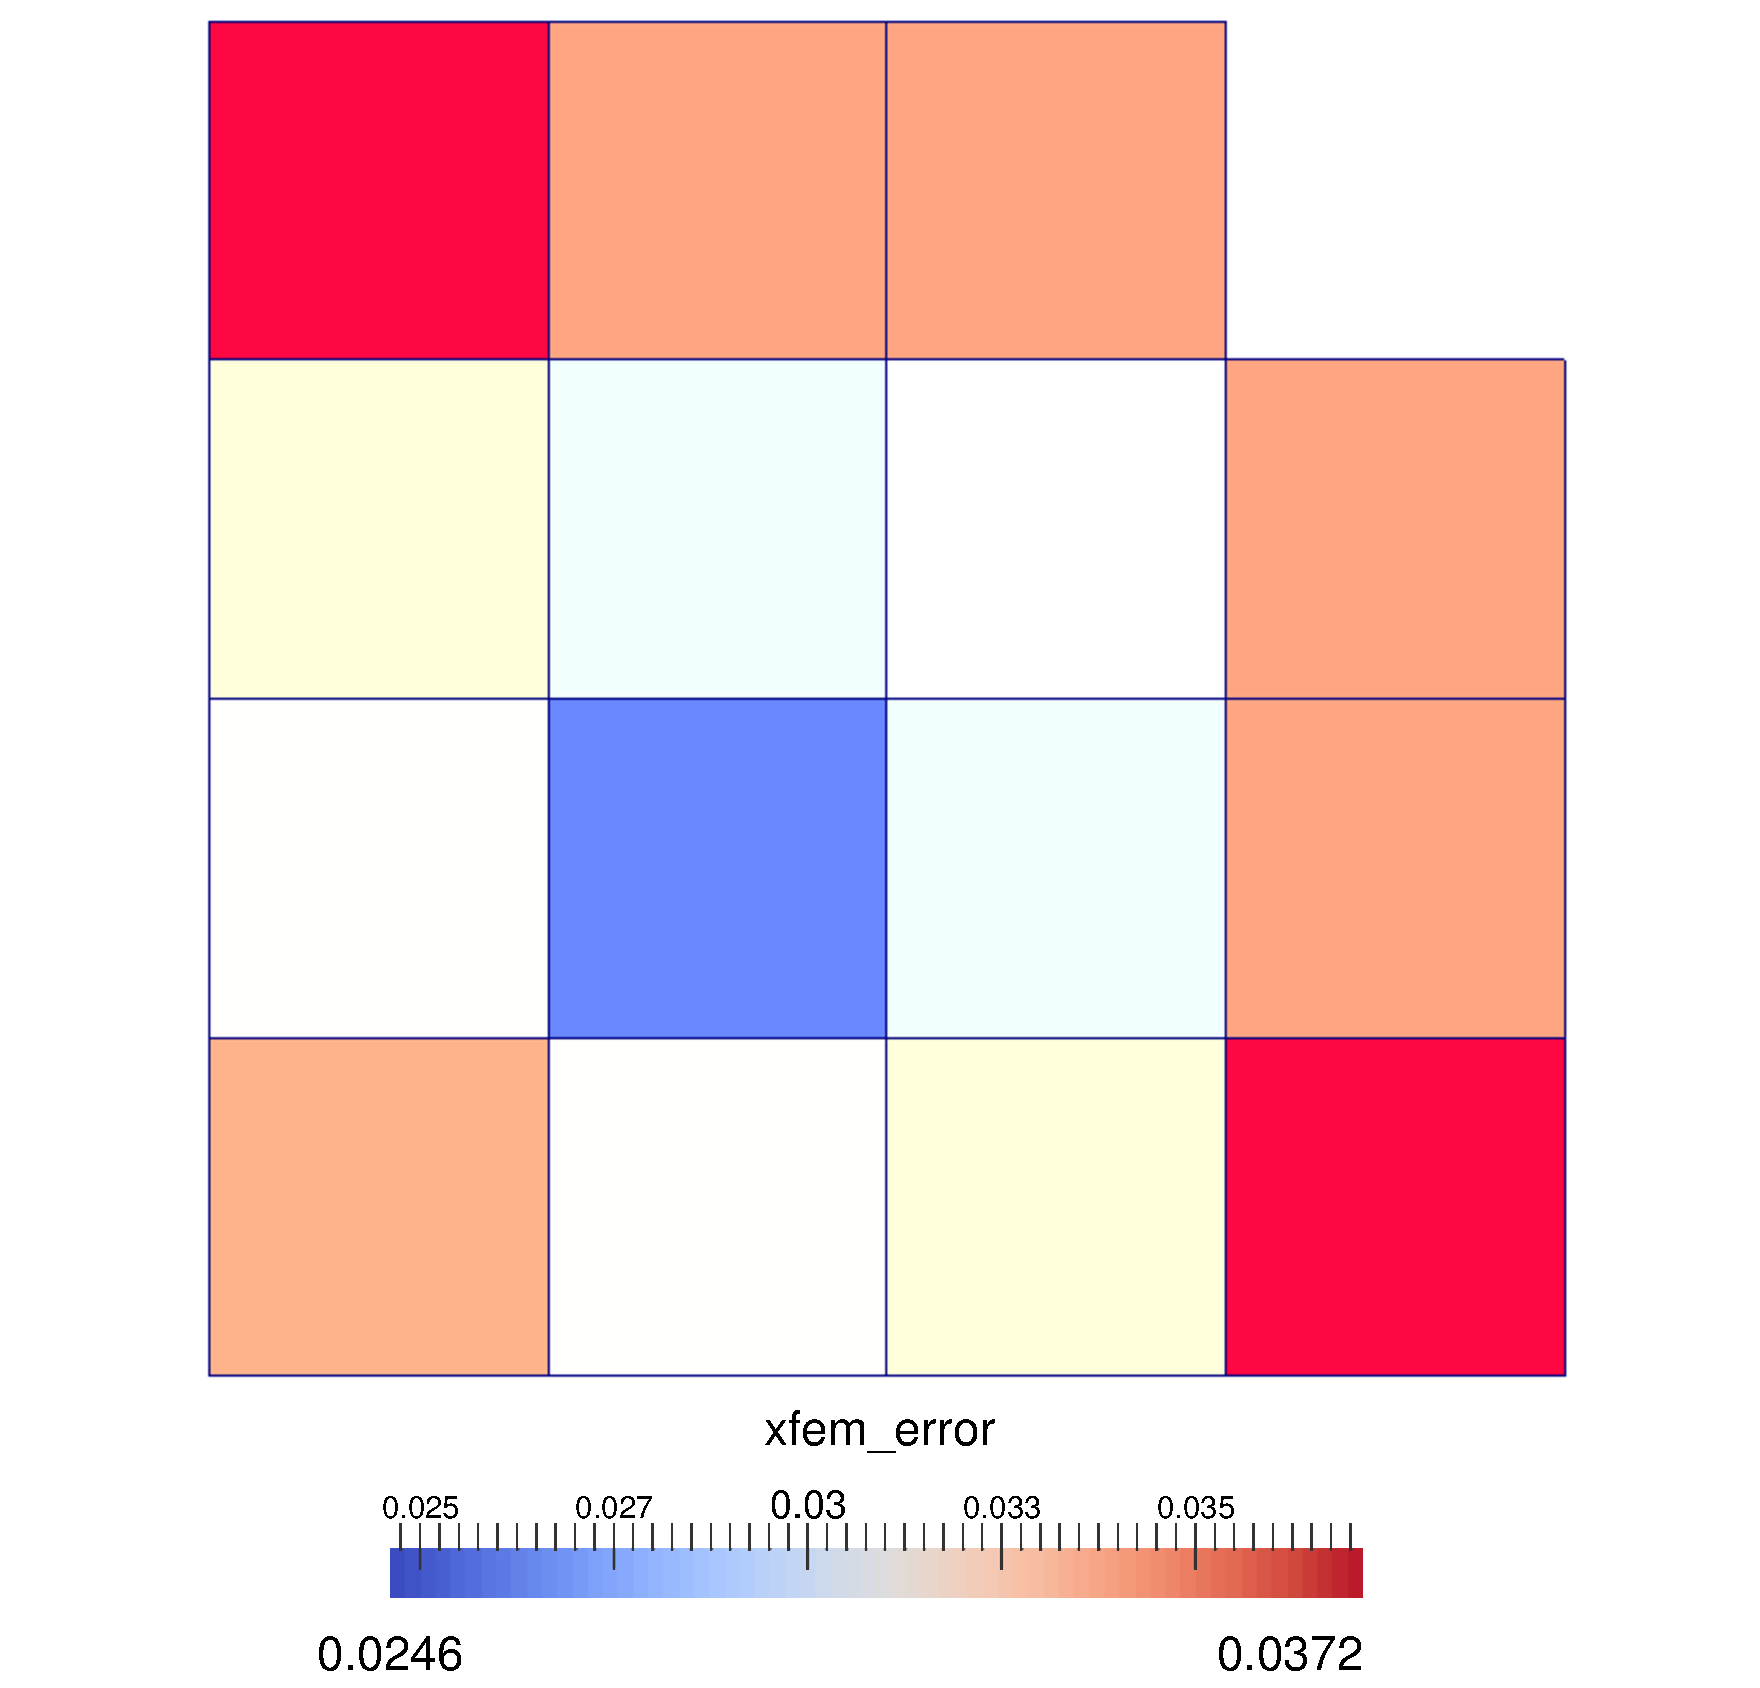
\includegraphics[width=0.45\textwidth]{results/adaptive_refinement_extract_3_new.pdf} }
  \caption[Adaptive refinement comparision]
  {Comparision of elementwise error in $L_2$ norm using different refinement techniques.
  }
  \label{fig:adapt_refinement_norm}
\end{figure}


\subsection{Circle integration experiment}
The approximation of the integration domain is also the source of the error. We decided to run 
an experiment on integrating the characteristic function of the well with our adaptive integration.
The domain $\Omega$ is a square $4\times4$ out of which a circle of radius 1.0 is cut off. The characteristic 
function is considered
\begin{equation}
  \chi(\bx) = \left\{
    \begin{array}{l l}
      0 & \quad \textrm{if } \bx \textrm{ is inside the circle}\\
      1 & \quad \textrm{otherwise}
  \end{array} \right.
\end{equation}
and the integral 
\begin{equation}
  \int_{\Omega}\chi(\bx) \dd\bx = 4^2 - \pi
\end{equation}
is equal the area of the square minus the area of the circle.

In this experiment we investigate the influence of the order of the quadrature rule and the level of
the refinement on how precisely the well geometry is captured.

In the graph in \fig{fig:adapt_ref_convergence} we can see that for all the quadratures the convergence rate
is similar, around 1.5. The gain from using higher order quadratures is not worth, especially in case 
of the order 4 the error is not much smaller than the error of the quadrature of the order 3. 

Finally the highest level of refinement is chosen to be 10 and the quadrature order to be 3. The number of
the quadrature points generated by the process desribed above in \ref{sec:refinement_element} is then similar 
both in the original (14793) and improved version (14819).

\begin{figure}[!htb]
%   \vspace{0pt}
%TODO: add refinement level to legend
  \centering    
  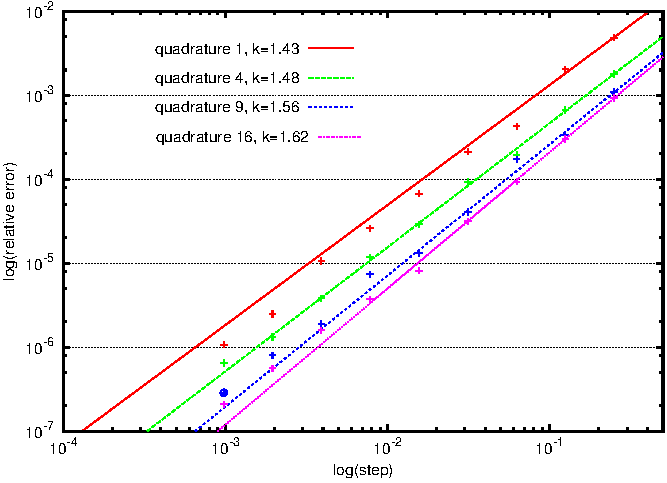
\includegraphics[width=0.7\textwidth]{results/adaptive_integration.pdf}
%   \subfloat[rozdìlený element s vrtem]{\label{fig:adapt_ref_a} 
%     \includegraphics[width=70mm]{\figpath adaptive_ref.pdf} }
%   \hspace{0pt}
%   \subfloat[detail hranice vrtu]{\label{fig:adapt_ref_b} 
%     \includegraphics[width=72mm]{\figpath adaptive_ref_detail.pdf} }
  \caption[Adaptive refinement convergence]{Convergence of adaptive refinement of a circle cutoff.}
  \label{fig:adapt_ref_convergence}
\end{figure}

%TODO:
% * non-optimal convergence rate with the approach of [gracie] and their integration scheme 3-4
% 
% * the above can be improved by using higher order quadrature rules (6-6)
% 
% * problem is that we do not represent the well edge and mainly its surrounding well enough

\section{Estimate the enrichment radius}
The enrichment is done in order to diminish approximation error of the precise solution of the problem, i.e.
$\tilde e_h = \min\limits_{u_h \in V_h} \| u - u_h \|_{V}$. Let us consider a well at origin, the radius $R$ of the 
enrichment should be chosen so that 
\[
   \min\limits_{u_h \in V^P_h} \| \log  \vc x - u_h\|_{V(\Omega^P)} \le \epsilon
\]
where $V^P_h$ is polynomial finite element approximation space on unenriched part $\Omega^P$ of the domain $\Omega$, 
$V = H^1(\Omega)$, and $\epsilon$ is prescribed tolerance. 

For linear elements and 1D case, we get
\begin{align*}
 \|\log x - u_h\|^2_{L^2(r,r+h)} 
 &= h\int_0^1 \abs{\log(r+ht) - \big[ (1-t)\log r + t\log(r+h) \big]}^2\d t\\
 &= \frac{h^5}{4r^4}\int_0^1 t^2(1-t)^2 + O(h^6)\approx \frac{h^5}{120 r^4}
\end{align*}

\begin{align*}
 \|\nabla (\log x - u_h)\|^2_{L^2(r,r+h)} &=
 h\int_0^1 \abs{\frac{1}{r+ht} - \frac{\log(r+h) - \log r}{h}}^2\d t \\
 &=
\frac{h^3}{r^4}\int_0^1 (\frac12-t)^2 + O(h^4)\approx 
\frac{h^3}{12 r^4}
\end{align*}

And thus,
\[
  \|\log x - u_h\|_{H^1(r,r+h)} \approx h^{3/2} r^{-2} 12^{-1/2}.
\]

Let us consider a 2D domain. The $H^1$ error on elements in distance $r$ is same as in the 1D case up to a constant close to 1 
(potrebuje numericke overeni). Thus error on the band at distance $r$ is proportional to 
\[
 \|\log \vc x - u_h\|^2_{H^1(\Omega^P)} \approx \int_R^{diam \Omega} 2\pi r \frac{h^3}{12 r^4} \d r \le \frac{2\pi h^3}{12} 
\frac{2}{R^2} \approx \frac{h^3}{R^2}.
\]
Then, the optimal choice of $R$ for given $H^1$ tolerance $\epsilon$ should be
\[
  R = \frac{h^{3/2}}{\epsilon}
\]


\section{Results}
\label{sec:results}

\subsection{Analytical solution}
To measure convergence an analytic solution is needed. 
%TODO: why only single aquifer problems
Let's start with a Laplace problem on a circular disk
with a single well in the center
\begin{eqnarray} \label{eqn:laplace_problem}
    -T \Delta h = 0 \nonumber\\
    h|_{\partial\Omega} = P_D \\
    h|_{B_w} = P_w \nonumber
\end{eqnarray}
where the pressure $P_w$ at the well edge $B_w$ and the pressure $P_D$ at the boundary are given.
Remind the function \eqref{eqn:solution_form} $h=\log(r_w)+b$ (which we used to define the enrichment function) 
and find the constants $a,b$ using the boundary conditions such that \eqref{eqn:solution_form} is the solution 
of \eqref{eqn:laplace_problem}.
We obtain $a,b$ by solving
\begin{eqnarray*}
  a\log(R_w) + b = P_w, \\
  a\log(R) + b = P_D,
\end{eqnarray*}
where $R$ is radius of the domain and $R_w$ is the well radius.
The solution of \eqref{eqn:laplace_problem}, which we shall use as the reference, is then
\begin{equation} \label{eqn:laplace_solution}
  h=a\log(r_w)+b \qquad \textrm{ with } a=\frac{P_w}{\log\left(\frac{R_w}{R}\right)}, \; b=-a\log R
\end{equation}

Second problem we solve is a Poisson problem
\begin{eqnarray} \label{eqn:poisson_problem}
    -T \Delta h = TU\omega^2\sin(\omega x) \nonumber\\
    h|_{\partial\Omega} = P_D + U\sin(\omega x)\\
    h|_{B_w} = P_w. \nonumber
\end{eqnarray}
where $U$ and $\omega$ are given
%where $U$ is the amplitude and $\omega$ is the angular frequency 
and the solution 
\begin{equation} \label{eqn:poisson_solution}
  h=a\log(r_w)+b+U\sin(\omega x),
\end{equation}
with $a,b$ being the same as in \eqref{eqn:laplace_solution}, is obtained the same way as above.

\subsection{Convergence on Laplace problem}
\subsection{Convergence on Poisson problem with sinusoidal source}

\section{Summary}
\label{sec:summary}

\section{Acknowledgement}
This work was made under the sincere guidance and support of Mgr. Jan B{\v r}ezina, Ph.D.

This work was supported by the Ministry of Education of the Czech Republic within the SGS project 
no. 21066/115 on the Technical University of Liberec.

%% The Appendices part is started with the command \appendix;
%% appendix sections are then done as normal sections
%% \appendix

%% \section{}
%% \label{}

%% If you have bibdatabase file and want bibtex to generate the
%% bibitems, please use
%%
%%  \bibliographystyle{elsarticle-harv} 
%%  \bibliography{<your bibdatabase>}

%% else use the following coding to input the bibitems directly in the
%% TeX file.

% \begin{thebibliography}{00}
% 
% %% \bibitem[Author(year)]{label}
% %% Text of bibliographic item
% 
% \bibitem[ ()]{}
% 
% \end{thebibliography}
 %\nocite{dip}
 %\bibliographystyle{elsarticle-harv} 
 %\bibliographystyle{elsarticle-num-names} 
 \bibliographystyle{elsarticle-num} 
 \bibliography{../citace.bib}
\end{document}

\endinput
%%
%% End of file `elsarticle-template-harv.tex'.
